\chapter{Expenditure Multipliers (Text Ch. 27)}

\section{Fixed prices and expenditure plans}

The \emph{Keynesian model} describes the economy in the very short run, when prices are
fixed. Firms do not change their prices; they meet whatever demand arises at those prices.
Because the price level is fixed, \emph{aggregate demand alone determines real GDP} in this
model. The model explains how changes in spending are \emph{multiplied}, and it underlies
the AD curve.

\subsection{Expenditure plans}

The components of aggregate expenditure sum to real GDP:
\[
  Y = C + I + G + X - M.
\]
Two of these components, consumption and imports, depend on real GDP itself. This
two-way link (expenditure determines GDP, and GDP determines expenditure) is the key to
the model.

\subsection{The consumption function and saving function}

\emph{Disposable income} ($YD$) is aggregate income minus net taxes ($YD = Y - T$).
Households either spend it on consumption or save it:
\[
  YD = C + S.
\]

\begin{definition}[Consumption and saving functions]
The \emph{consumption function} is the relationship between consumption expenditure and
disposable income, other things remaining the same. The \emph{saving function} is the
relationship between saving and disposable income. In linear form,
\[
  C = a + b\,YD, \qquad S = -a + (1 - b)\,YD,
\]
where $a$ is \emph{autonomous consumption} (consumption when $YD = 0$, financed by
dissaving) and $b$ is the marginal propensity to consume.
\end{definition}

Other influences on consumption and saving, which \emph{shift} these functions, include
the real interest rate, wealth, expected future income and the price level.

\subsection{Marginal propensities to consume and save}

\begin{definition}[MPC and MPS]
The \emph{marginal propensity to consume} (MPC) is the fraction of a change in disposable
income that is spent on consumption; the \emph{marginal propensity to save} (MPS) is the
fraction that is saved:
\[
  MPC = \frac{\Delta C}{\Delta YD}, \qquad MPS = \frac{\Delta S}{\Delta YD}.
\]
\end{definition}

\begin{proposition}
$MPC + MPS = 1$.
\end{proposition}
\begin{proof}
Since $\Delta C + \Delta S = \Delta YD$, dividing by $\Delta YD$ gives
$\dfrac{\Delta C}{\Delta YD} + \dfrac{\Delta S}{\Delta YD} = 1$.
\end{proof}

\begin{example}
Let $C = 100 + 0.75\,YD$. Then $S = YD - C = -100 + 0.25\,YD$, so $MPC = 0.75$ and
$MPS = 0.25$.
\begin{center}
\begin{tabular}{ccc}
\toprule
$YD$ & $C$ & $S$ \\
\midrule
0 & 100 & $-100$ \\
200 & 250 & $-50$ \\
400 & 400 & 0 \\
800 & 700 & 100 \\
\bottomrule
\end{tabular}
\end{center}
At $YD = 400$ households consume all their income (saving is zero); below that they
dissave.
\end{example}

\begin{center}
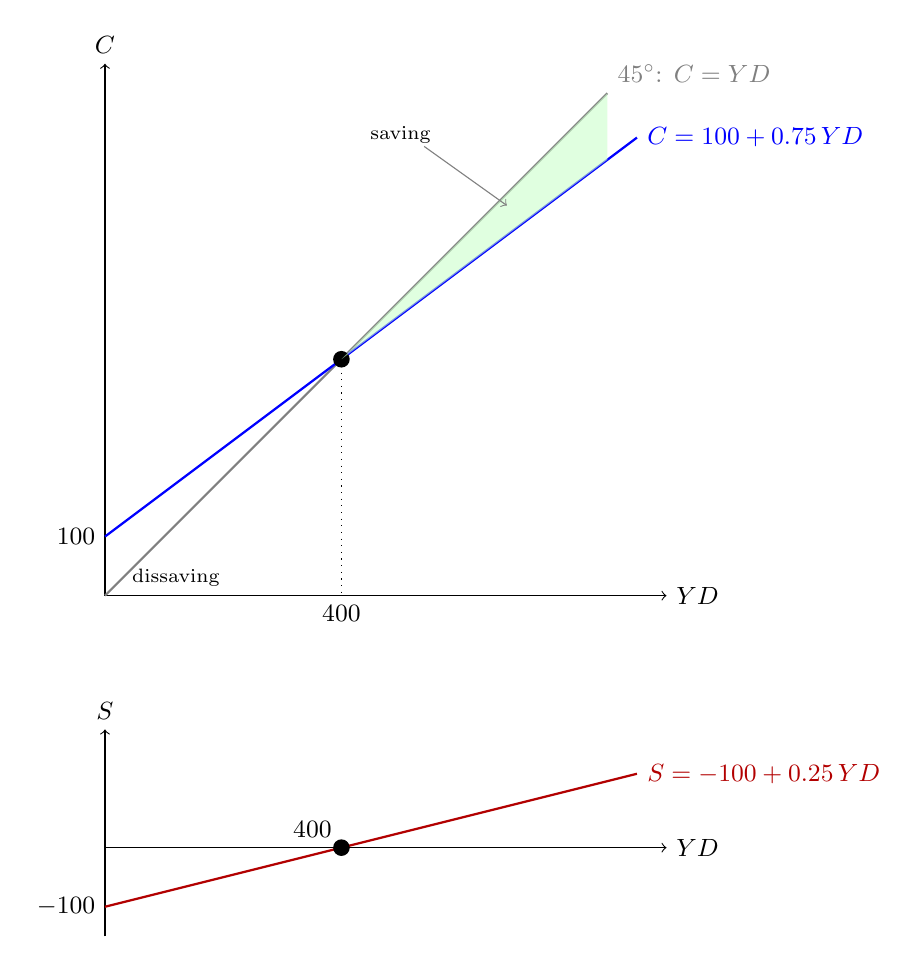
\begin{tikzpicture}[x=0.0075cm, y=0.0075cm, every node/.style={font=\small}]
  \draw[->] (0,0) -- (950,0) node[right] {$YD$};
  \draw[->] (0,0) -- (0,900) node[above] {$C$};
  \draw[gray, thick] (0,0) -- (850,850) node[above right] {$45^\circ$: $C = YD$};
  \draw[thick, blue] (0,100) -- (900,775) node[right] {$C = 100 + 0.75\,YD$};
  \fill (400,400) circle (3pt);
  \draw[dotted] (400,400) -- (400,0) node[below] {400};
  \node[left] at (0,100) {100};
  \fill[green!20, opacity=0.6] (400,400) -- (850,850) -- (850,737.5) -- cycle;
  \node[font=\scriptsize] at (500,780) {saving};
  \node[font=\scriptsize, align=center] at (120,30) {dissaving};
  \draw[->, gray] (540,760) -- (680,660);
  \begin{scope}[yshift=-3.2cm]
    \draw[->] (0,0) -- (950,0) node[right] {$YD$};
    \draw[->] (0,-150) -- (0,200) node[above] {$S$};
    \draw[thick, red!70!black] (0,-100) -- (900,125) node[right] {$S = -100 + 0.25\,YD$};
    \fill (400,0) circle (3pt) node[above left] {400};
    \node[left] at (0,-100) {$-100$};
  \end{scope}
\end{tikzpicture}
\end{center}
The consumption function crosses the $45^\circ$ line at $YD = 400$, where saving is zero.
To the right, the vertical gap between the $45^\circ$ line and $C$ is saving; to the left,
households dissave. The slopes are $MPC = 0.75$ and $MPS = 0.25$.

\subsection{Imports}

Imports increase with real GDP. The \emph{marginal propensity to import} ($m$) is the
fraction of an increase in real GDP spent on imports: $m = \Delta M/\Delta Y$.

\section{Real GDP with a fixed price level}

\begin{definition}[Aggregate planned expenditure]
\emph{Aggregate planned expenditure} (AE) is the sum of planned consumption expenditure,
planned investment, planned government expenditure and planned exports, minus planned
imports.
\end{definition}

\begin{definition}[Autonomous and induced expenditure]
\emph{Autonomous expenditure} ($A$) is the part of aggregate expenditure that does not
change when real GDP changes: investment, government expenditure, exports, and the
autonomous parts of consumption and imports. \emph{Induced expenditure} is the part that
does change with real GDP: consumption expenditure minus imports, to the extent they
depend on income.
\end{definition}

\begin{important}[Pitfall]
Autonomous expenditure is not simply ``$C + I + G + X$''. Most of $C$ is induced
(it varies with income); only autonomous consumption $a$ belongs in $A$, along with
$I$, $G$ and $X$.
\end{important}

\subsection{The AE curve}

Combining, the AE curve is a straight line
\[
  AE = A + (\text{slope})\,Y,
\]
where the slope is the extra induced spending per extra dollar of real GDP. With no
income taxes and no imports, the slope is the MPC. With an income tax rate $t$ (so
$YD = (1 - t)Y$) and marginal propensity to import $m$,
\[
  \text{slope of AE} = b(1 - t) - m.
\]

\subsection{Actual expenditure, planned expenditure and real GDP}

\emph{Actual} aggregate expenditure is always equal to real GDP (it includes unplanned
changes in inventories). \emph{Planned} expenditure need not equal real GDP.
\begin{itemize}
  \item If $AE > Y$, firms sell more than they produce; inventories fall unexpectedly,
        and firms increase production.
  \item If $AE < Y$, unsold goods pile up (unplanned inventory investment); firms cut
        production.
\end{itemize}

\begin{definition}[Equilibrium expenditure]
\emph{Equilibrium expenditure} is the level of aggregate expenditure that occurs when
aggregate planned expenditure equals real GDP. Graphically it is where the AE curve
crosses the $45^\circ$ line (the \emph{Keynesian cross}).
\end{definition}

\begin{theorem}[Equilibrium real GDP]
If $AE = A + sY$ with slope $0 < s < 1$, equilibrium real GDP is
\[
  Y^{*} = \frac{A}{1 - s}.
\]
\end{theorem}
\begin{proof}
Set $Y = AE = A + sY$, so $(1 - s)Y = A$.
\end{proof}

\begin{example}[A simple economy]
No government, no trade: $C = 100 + 0.75Y$ and $I = 200$. Then $AE = 300 + 0.75Y$, so
$Y^{*} = 300/(1 - 0.75) = 1200$. Check: $C = 100 + 900 = 1000$, $AE = 1000 + 200 = 1200$.
At $Y = 1000$, $AE = 300 + 750 = 1050 > 1000$: inventories fall by 50 and firms expand
output. At $Y = 1400$, $AE = 300 + 1050 = 1350 < 1400$: inventories pile up by 50 and
firms cut output.
\end{example}

\begin{center}
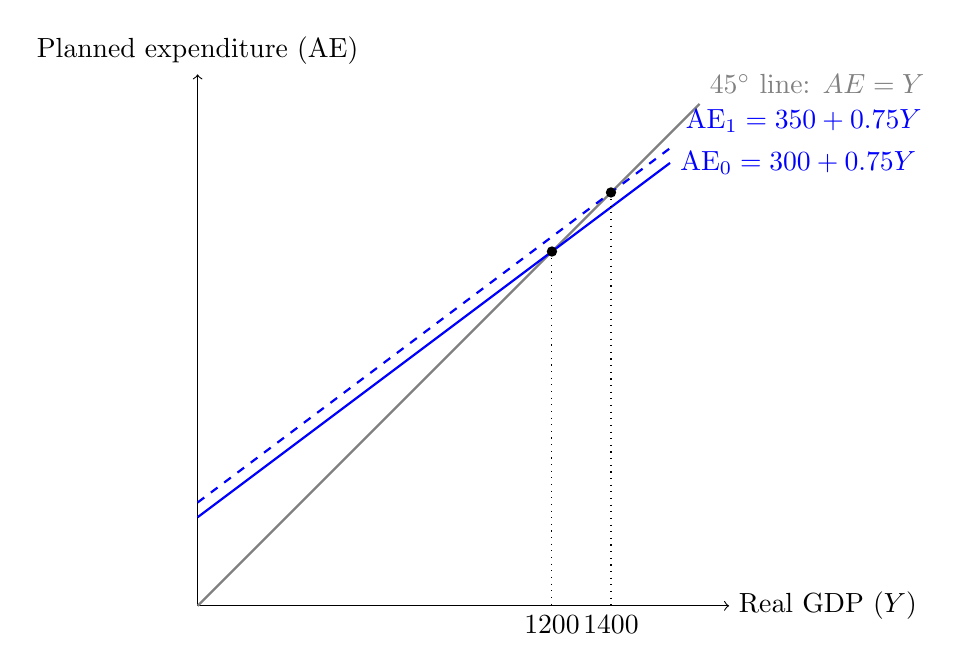
\begin{tikzpicture}[scale=0.75]
  \draw[->] (0,0) -- (9,0) node[right] {Real GDP ($Y$)};
  \draw[->] (0,0) -- (0,9) node[above] {Planned expenditure (AE)};
  \draw[thick, gray] (0,0) -- (8.5,8.5) node[above right] {$45^\circ$ line: $AE = Y$};
  \draw[thick, blue] (0,1.5) -- (8,7.5) node[right] {AE$_0 = 300 + 0.75Y$};
  \draw[thick, blue, dashed] (0,1.75) -- (8,7.75) node[above right=2pt] {AE$_1 = 350 + 0.75Y$};
  \fill (6,6) circle (2.5pt);
  \fill (7,7) circle (2.5pt);
  \draw[dotted] (6,6) -- (6,0) node[below] {1200};
  \draw[dotted] (7,7) -- (7,0) node[below] {1400};
\end{tikzpicture}
\end{center}

\section{The multiplier}

\begin{definition}[Multiplier]
The \emph{multiplier} is the amount by which a change in autonomous expenditure is
magnified or multiplied to determine the change in equilibrium expenditure and real GDP:
\[
  \text{multiplier} = \frac{\Delta Y}{\Delta A}.
\]
\end{definition}

\subsection{Why is the multiplier greater than 1?}

An increase in autonomous expenditure increases real GDP and therefore income. The extra
income induces extra consumption, which raises income again, and so on. Each round is
smaller than the last because part of each increase in income leaks out into saving
(and, in a fuller model, taxes and imports).

\begin{example}[The multiplier process]
In the simple economy, investment rises by 50 (to 250). Round by round, with $MPC = 0.75$:
\[
  \Delta Y = 50 + 37.5 + 28.125 + 21.09 + \cdots
  = 50\,(1 + 0.75 + 0.75^2 + \cdots) = \frac{50}{1 - 0.75} = 200.
\]
New equilibrium: $AE = 350 + 0.75Y$, so $Y^{*} = 350/0.25 = 1400$, an increase of 200.
The multiplier is $200/50 = 4$.
\end{example}

\begin{center}
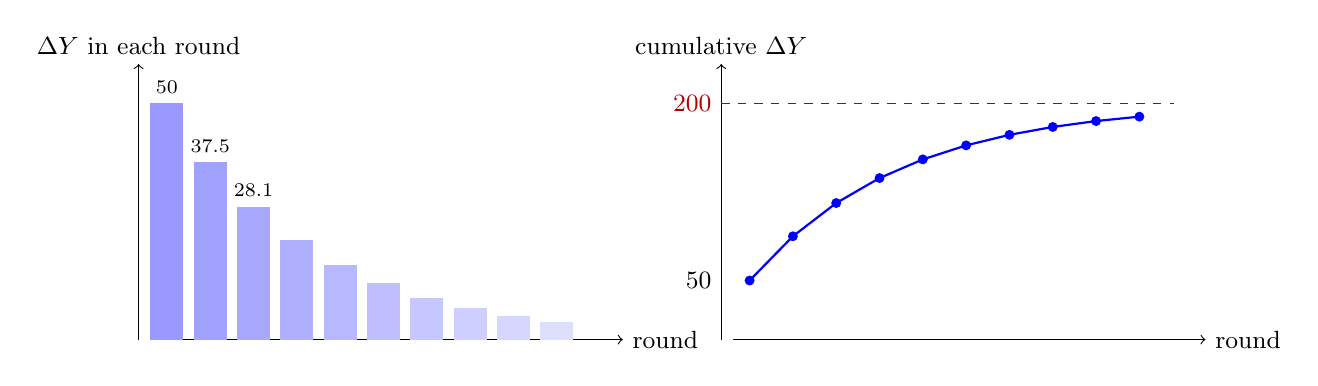
\begin{tikzpicture}[every node/.style={font=\small}]
  \draw[->] (0,0) -- (6,0) node[right] {round};
  \draw[->] (-0.15,0) -- (-0.15,3.5) node[above] {$\Delta Y$ in each round};
  \fill[blue!40] (0.00,0) rectangle (0.42,3.000);
  \fill[blue!37] (0.55,0) rectangle (0.97,2.250);
  \fill[blue!34] (1.10,0) rectangle (1.52,1.688);
  \fill[blue!31] (1.65,0) rectangle (2.07,1.266);
  \fill[blue!28] (2.20,0) rectangle (2.62,0.949);
  \fill[blue!25] (2.75,0) rectangle (3.17,0.712);
  \fill[blue!22] (3.30,0) rectangle (3.72,0.534);
  \fill[blue!19] (3.85,0) rectangle (4.27,0.400);
  \fill[blue!16] (4.40,0) rectangle (4.82,0.300);
  \fill[blue!13] (4.95,0) rectangle (5.37,0.225);
  \node[above, font=\scriptsize] at (0.21,3.0) {50};
  \node[above, font=\scriptsize] at (0.76,2.25) {37.5};
  \node[above, font=\scriptsize] at (1.31,1.69) {28.1};
  \begin{scope}[xshift=7.4cm]
    \draw[->] (0,0) -- (6,0) node[right] {round};
    \draw[->] (-0.15,0) -- (-0.15,3.5) node[above] {cumulative $\Delta Y$};
    \draw[dashed, red!70!black] (-0.15,3) node[left] {200} -- (5.6,3);
    \draw[thick, blue] (0.21,0.750) -- (0.76,1.312) -- (1.31,1.734) -- (1.86,2.051) -- (2.41,2.288) -- (2.96,2.466) -- (3.51,2.600) -- (4.06,2.700) -- (4.61,2.775) -- (5.16,2.831);
    \foreach \p in {(0.21,0.750),(0.76,1.312),(1.31,1.734),(1.86,2.051),(2.41,2.288),(2.96,2.466),(3.51,2.600),(4.06,2.700),(4.61,2.775),(5.16,2.831)} \fill[blue] \p circle (1.8pt);
    \node[left] at (-0.15,0.75) {50};
  \end{scope}
\end{tikzpicture}
\end{center}
Each round is $0.75$ of the one before (left); the running total approaches
$50/(1-0.75) = 200$ (right).

\subsection{The size of the multiplier and the slope of the AE curve}

\begin{theorem}
\[
  \text{multiplier} = \frac{1}{1 - \text{slope of AE curve}}.
\]
With no taxes or imports, the slope is the MPC, so the multiplier is
$\dfrac{1}{1 - MPC} = \dfrac{1}{MPS}$. With income taxes and imports,
\[
  \text{multiplier} = \frac{1}{1 - [\,b(1 - t) - m\,]}.
\]
\end{theorem}
\begin{proof}
From $Y^{*} = A/(1 - s)$, a change $\Delta A$ changes $Y^{*}$ by $\Delta A/(1 - s)$.
\end{proof}

\begin{example}[A full model]
$C = 100 + 0.75\,YD$, income tax rate $t = 0.2$ (so $YD = 0.8Y$), $I = 200$, $G = 300$,
$X = 150$, $M = 0.1Y$.
\begin{align*}
  AE &= 100 + 0.75(0.8Y) + 200 + 300 + 150 - 0.1Y \\
     &= 750 + (0.6 - 0.1)Y = 750 + 0.5Y.
\end{align*}
So $Y^{*} = 750/(1 - 0.5) = 1500$, and the multiplier is $1/(1 - 0.5) = 2$. Check:
$YD = 1200$, $C = 100 + 900 = 1000$, $M = 150$, and
$AE = 1000 + 200 + 300 + 150 - 150 = 1500$. Taxes are $0.2 \times 1500 = 300 = G$ (a
balanced budget) and $X = M$.

Comparing with the simple economy (multiplier 4): income taxes and imports
\emph{reduce} the multiplier, because part of each extra dollar of income goes to taxes
and to foreign goods instead of to Canadian consumption.
\end{example}

\begin{important}[Pitfall]
The multiplier uses the slope of the AE curve, not the MPC, whenever there are income
taxes or induced imports. In Canada, with substantial taxes and an import share near 30\%,
real-world multipliers are much smaller than $1/(1 - MPC)$, roughly 1 to 1.5.
\end{important}

\subsection{Business cycle turning points}

At a peak or trough, a small change in autonomous expenditure (often investment or
exports) is multiplied into a larger swing in real GDP. A recession begins when
autonomous spending falls and the multiplier amplifies the fall; an expansion begins when it
rises.

\begin{remark}[Paradox of thrift]
If everyone tries to save more (a fall in autonomous consumption), AE shifts down and
equilibrium real GDP falls by a multiple of the decrease; total saving may not rise at
all. What is prudent for one household can be harmful for the economy as a whole (the
fallacy of composition).
\end{remark}

\section{The multiplier and the price level}

In reality firms do change prices, so we connect the Keynesian model to the AS--AD model.

\subsection{Deriving the AD curve}

The AE curve is drawn for a given price level. A rise in the price level decreases
planned expenditure (wealth effect, intertemporal and international substitution), so the
AE curve shifts downward and equilibrium expenditure falls. Plotting the equilibrium real
GDP for each price level traces out the downward-sloping AD curve.

\begin{center}
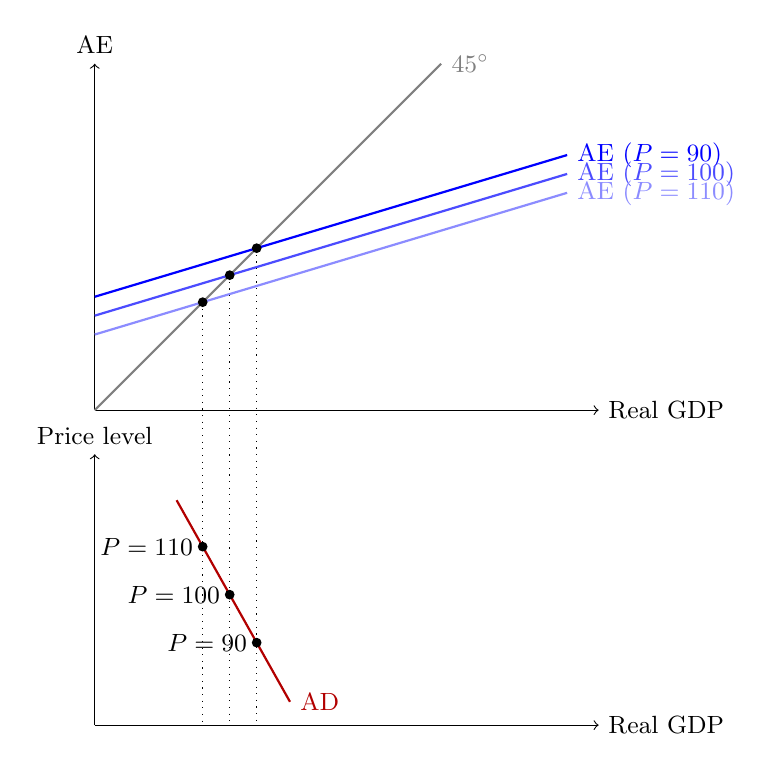
\begin{tikzpicture}[scale=0.8, every node/.style={font=\small}]
  % top: AE diagram
  \draw[->] (0,5) -- (8,5) node[right] {Real GDP};
  \draw[->] (0,5) -- (0,10.5) node[above] {AE};
  \draw[gray, thick] (0,5) -- (5.5,10.5) node[right] {$45^\circ$};
  \draw[thick, blue] (0,6.8) -- (7.5,9.05) node[right] {AE ($P = 90$)};
  \draw[thick, blue!70] (0,6.5) -- (7.5,8.75) node[right] {AE ($P = 100$)};
  \draw[thick, blue!45] (0,6.2) -- (7.5,8.45) node[right] {AE ($P = 110$)};
  \fill (2.571,7.571) circle (2.2pt); \fill (2.143,7.143) circle (2.2pt); \fill (1.714,6.714) circle (2.2pt);
  \draw[dotted] (1.714,6.714) -- (1.714,0);
  \draw[dotted] (2.143,7.143) -- (2.143,0);
  \draw[dotted] (2.571,7.571) -- (2.571,0);
  % bottom: AD
  \draw[->] (0,0) -- (8,0) node[right] {Real GDP};
  \draw[->] (0,0) -- (0,4.3) node[above] {Price level};
  \draw[thick, red!70!black] (1.3,3.57) -- (3.1,0.37) node[right] {AD};
  \fill (1.714,2.833) circle (2.2pt) node[left] {$P = 110$};
  \fill (2.143,2.071) circle (2.2pt) node[left] {$P = 100$};
  \fill (2.571,1.309) circle (2.2pt) node[left] {$P = 90$};
\end{tikzpicture}
\end{center}
Each price level gives its own AE curve (top); a higher price level lowers planned
expenditure and the equilibrium real GDP. Plotting each equilibrium against its price level
traces out the AD curve (bottom).

\subsection{Changes in aggregate expenditure and AD}

A change in autonomous expenditure \emph{not} caused by the price level shifts the AE curve
and shifts the AD curve horizontally by the multiplier times the change in autonomous
expenditure.

\subsection{Equilibrium real GDP and the price level}

In the short run, the SRAS curve slopes upward, so when AD increases the price level
rises too. The higher price level shifts the AE curve back down part of the way, so the
increase in real GDP is \emph{smaller} than the multiplier effect at a fixed price level.
In the long run, real GDP returns to potential and the increase in AD only raises the
price level: the long-run multiplier on real GDP is zero.

\begin{example}
In the full model, exports rise by 40. At a fixed price level, AD shifts right by
$2 \times 40 = 80$. Because SRAS slopes up, the price level rises and real GDP increases
by less than 80 in the short run (say 50). In the long run, money wages rise until real GDP
is back at potential.
\end{example}

\section{Summary}

\begin{itemize}
  \item With fixed prices, aggregate planned expenditure determines real GDP.
  \item $C = a + b\,YD$, $S = -a + (1 - b)\,YD$, $MPC + MPS = 1$; imports rise with real
        GDP at rate $m$.
  \item $AE = A + sY$, with slope $s = b(1 - t) - m$; equilibrium where $AE = Y$:
        $Y^{*} = A/(1 - s)$. Unplanned inventory changes push the economy there.
  \item Multiplier $= \Delta Y/\Delta A = 1/(1 - s)$; equals $1/MPS$ with no taxes or
        imports. Taxes and imports make it smaller.
  \item The AE model derives the AD curve; a change in autonomous expenditure shifts AD by
        the multiplier times the change. With upward-sloping SRAS the real GDP effect is
        smaller, and zero in the long run.
\end{itemize}
